
The challenge that this dataset poses for the identification of causal effects of FDI is that the treatment (FDI) is not assigned randomly across firms but the result of a selection process. Investors will carefully decide which firms to invest in. Thus, treatment allocation will likely depend on observable firm characteristics in 2015, such that firms in the treatment group will structurally differ from firms in the untreated group. Table \ref{sumstat_treatment} shows that in the available dataset this imbalance in pre-treatment characteristics between treated and non-treated firms can be found across all available performance indicators from 2015. In addition, Table \ref{selection_logit} presents the result of a logit regression of FDI on pre-treatment characteristics, which corroborates the statistical significance of correlations with FDI assignment for all available pre-treatment variables except log wages. The set of pre-treatment firm characteristics is, consequently, correlated with post-treatment performance as well as with treatment allocation, which violates the conditional independence assumption necessary for causal identification. As this violation is found across multiple variables, the data suffers from what is called \textit{the curse of dimensionality}. This can be circumvented by propensity score matching such that causal identification of FDI effects on firm performance can still be achieved.\\ \par 

 \begin{table}[htbp]\centering
\def\sym#1{\ifmmode^{#1}\else\(^{#1}\)\fi}
\caption{Logit estimation results of FDI on pre-treatment observables \label{selection\_logit}}
\begin{tabular}{l*{1}{cc}}
\hline\hline
                &\multicolumn{2}{c}{(1)}\\
                &\multicolumn{2}{c}{FDI/TREATMENT dummy in 2016}\\
                &        b   &       se\\
\hline
FDI/TREATMENT dummy in 2016&            &         \\
Wages in 2015 (logs)&  -0.0008   &  (0.008)\\
Total factor productivity in 2015&  -0.0917***&  (0.016)\\
Employment in 2015 (logs)&   0.1905***&  (0.011)\\
Export intensity in 2015&  47.2347***&  (0.765)\\
Debt in 2015 (logs)&  -0.3426***&  (0.109)\\
RD in 2015 (dummy)=0&   0.0000   &      (.)\\
RD in 2015 (dummy)=1&   0.2892***&  (0.097)\\
Low-tech        &   0.0000   &      (.)\\
Medium low      &  -2.1258***&  (0.104)\\
Medium high     &  -5.0274***&  (0.112)\\
High-tech       &  -8.5163***&  (0.164)\\
 Listed companies&   0.0000   &      (.)\\
 Subsidiaries   &   1.8301***&  (0.148)\\
 Independent    &   3.4707***&  (0.150)\\
 State          &   2.1772***&  (0.151)\\
No ports within 500km&   0.0000   &      (.)\\
Ports within 500km&  -3.0085***&  (0.087)\\
Constant        &  -7.0707***&  (0.212)\\
\hline
Observations    &    11323   &         \\
\hline\hline
\end{tabular}
\end{table}



% check balancedness computationally, check significance of all variables
 
 In order for propensity score matching to successfully alleviate any concerns of selection bias, a scoring function needs to be identified that achieves balancedness in terms of relevant observables, on the one hand, and a good common support, i.e. overlap on the other. This is not trivial. Imagine a situation in which treatment is assigned according to one specific set of variables, z. All subjects receiving treatment exhibit high values in z. If scoring is performed based on this variable set z propensity scores will be high for firms with high values of z and matching of firms with similar propensity scores will produce very little differences in values of z. Yet, this will produce a most certainly bad overlap. Opposed to that using a variable that is not related to treatment assignment for the propensity score matching will produce a high overlap as propensity scores calculated based on an unrelated variable will be similarly distributed within treatment and non-treatment groups, but it will be unlikely that this matching procedure will be able to balance the previously unbalanced variables. Consequently, a scoring function specification has to be found that balances all variables relevant for treatment assignment but in a way that produces high overlap. \\ \par 
 
 In a simple logit regression, almost all pre-treatment performance indicators showed relevance for selection. Figure \ref{ol_linlog1} shows the overlap and Table \ref{bal_linlog1} the balancedness check results of a linear functional specification including all these variables in a logit scoring function. It can be seen that this functional specification is not suited to achieve sample balance in a 1 on 1 matching procedure and does not provide sufficient overlap to identify an unbiased average treatment effect. Varying the functional specification in multiple ways (using probit instead of logit, interacting continuous performance indicators with categorical variables) does not produce any considerable improvement in overlap (compare Figure \ref{ol_intlog1} and \ref{ol_intprob1} in the Appendix). If we reduce the number of variables used in the scoring function to a subset of the pre-treatment observables, we find improvements in overlap as is expected based on the above presented argument (compare e.g. Figure \ref{ol_linlog1_red}). However, this comes at the cost of missing control over several variables that could be shown to significantly drive selection. In an attempt to reduce dimensionality of the information used while keeping control over all variables relevant for selection we opt for translating continuous performance indicators into less fine-grained categorical variables. In particular, we construct a variable "EXP2015\_CAT" that assigns the values 0, 1 or 2 for firms that have an export intensity of 0, below 25\% or larger 25\%, respectively. Using a scoring function in which the remaining continuous variables are interacted with the binary/ categorical variables including "EXP2015\_CAT" achieves strong improvements in overlap compared to the other specifications based on the full set of variables (see Figure \ref{ol_intcatlog1}). In addition, we find acceptable balancedness levels in the 1 on 1 matching, with matched differences of close to or above 0.2 in only two cases (compare Table \ref{bal_intcatlog1}). Testing various alternative matching specifications such as matching with the two or four nearest neighbours or using a caliper (compare Tables \ref{bal_intcatlog2} and \ref{bal_intcatlog4} in the Appendix) shows that the best results are indeed achieved in a 1 on 1 matching. \\ \par

\begin{table}
	\centering
		\caption{Balance check of the propensity scoring using a logit model (linear variable inclusion) and a 1 on 1 matching procedure}
	\label{bal_linlog1}
\begin{tabular}{lcccc}
	\hline \hline
	                    &    r(table)&            &            &            \\
                    &    Diff:Raw&  Diff:Match&   Ratio:Raw& Ratio:Match\\
log wages in 2015   &   -.1300321&   -.0515036&    .9769191&    .8845742\\
Total factor productivity in 2015&    -.178877&    .2139231&    .9473458&    .4003003\\
log of employment in 2015&    .5654306&    -.156559&     .803081&    .6229867\\
EXPORT INTENSITY in 2015&    1.014184&    .5934387&    1.228659&    1.336483\\
 log of DEBTS in 2015&   -.0529435&   -.2515877&    1.051101&    1.021671\\
R\&D dummy in 2015=1&    .0356507&   -.0076941&    1.085768&    .9795245\\
Medium low-tech industries&    .1206088&   -.0152956&    1.263082&    .9634731\\
Medium high-tech industries&   -.2329159&   -.1939862&    .8156583&    .7717778\\
High-tech industries&   -.5425507&    .4301909&    .2855456&    1.693899\\
 Subsidiaries       &    -.018354&    -.088095&    .9769702&     .858366\\
 Independent        &    .0616272&   -.0365731&     1.02321&    .9742405\\
 State              &    .1016402&   -.4001546&    1.100951&    .7088027\\
Ports within 500km  &    .4092869&   -.3412843&    1.253595&    .8230184\\

	\hline \hline
\end{tabular}
\end{table}

\begin{figure}
	\centering
	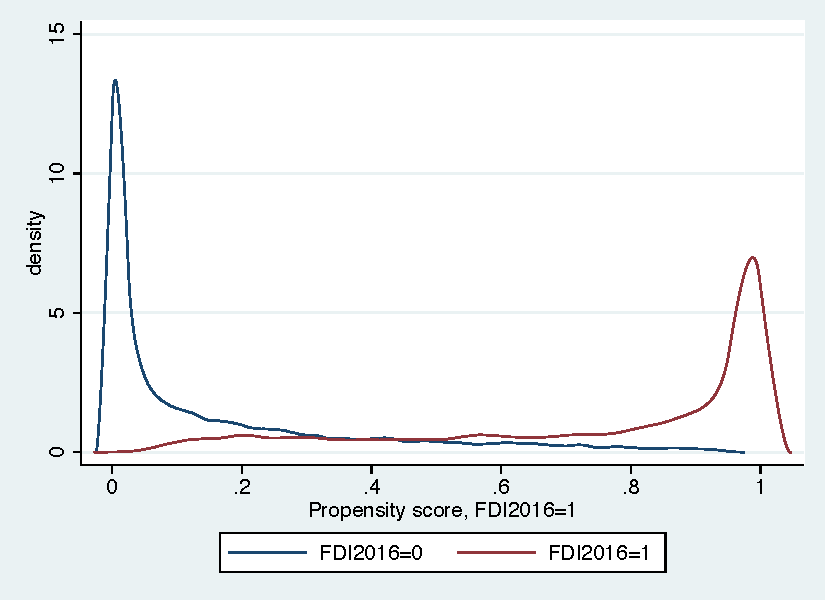
\includegraphics[scale=0.6]{figures_and_tables/3_overlap_linearlogit1o1.pdf}\
	\caption{Overlap resulting from the propensity scoring using a logit model (linear variable inclusion).}
	\label{ol_linlog1}
\end{figure}

\begin{figure}
	\centering
	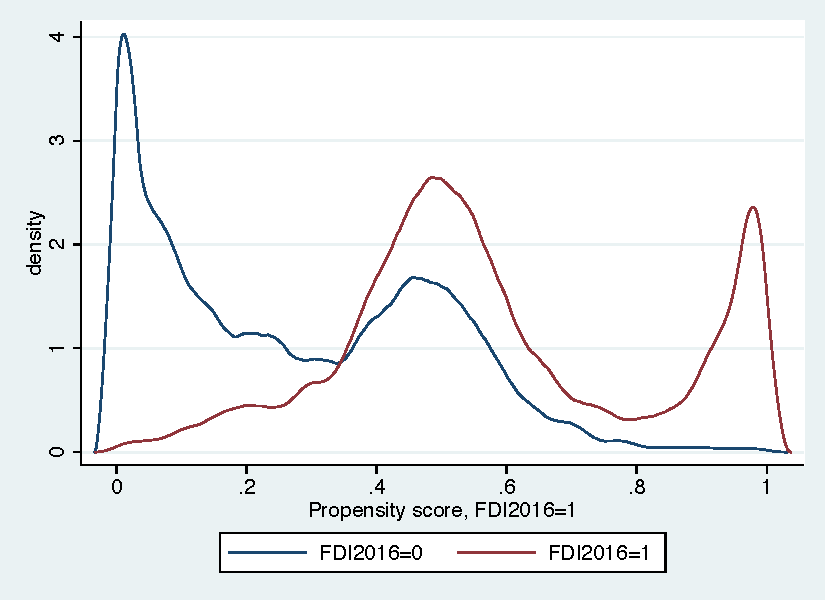
\includegraphics[scale=0.6]{figures_and_tables/3_overlap_intcatlogit1o1.pdf}\
	\caption{Overlap resulting from the propensity scoring using a logit model (interactions between the set of continuous variables excluding exports and the categorical/binary variables including exports)}
	\label{ol_intcatlog1}
\end{figure}

\begin{table}
	\centering
	\begin{tabular}{lcccc}
		\hline \hline
	 
            &    Diff:Raw&  Diff:Match&   Ratio:Raw& Ratio:Match\\ \hline
0b.RD2015xc.logwages2015&   -.1195646&    .0525046&     .947075&    1.062749\\
1.RD2015xc.logwages2015&    .0055913&    .0576109&    .9912599&    1.274914\\
1b.TECHxc.logwages2015&    .4099088&    .0288036&    1.446385&    1.012937\\
2.TECHxc.logwages2015&    .0985765&    .0376167&    1.221177&    1.078534\\
3.TECHxc.logwages2015&   -.1947846&   -.0195882&    .7998561&    1.077204\\
1b.OWNxc.logwages2015&   -.2416651&   -.0406993&    .3646025&    .8427318\\
2.OWNxc.logwages2015&   -.0501523&    -.078579&    .8787442&    .8758421\\
3.OWNxc.logwages2015&    .0095374&    .0352781&    .9615021&    1.109249\\
0b.PORTxc.logwages2015&   -.3780525&    .1273289&    .9245549&    1.141669\\
1b.EXP2015\_CATxc.logwages2015&   -.4723787&    .0947225&    1.179189&    1.081208\\
0b.RD2015xc.TFP2015&   -.1739665&   -.0203347&    .9100893&    .9091296\\
1.RD2015xc.TFP2015&    .0080044&    .0443347&    .9791256&    1.135322\\
1b.TECHxc.TFP2015&    .3830039&    .0387406&    1.517568&     1.02464\\
2.TECHxc.TFP2015&    .0592069&    .0218559&     1.09476&    1.039168\\
3.TECHxc.TFP2015&   -.2626395&   -.0332445&    .6142341&    .9655526\\
1b.OWNxc.TFP2015&   -.2670312&   -.0571476&    .2665297&     .720536\\
2.OWNxc.TFP2015&    -.064156&   -.0762223&    .8276227&    .8391969\\
3.OWNxc.TFP2015&   -.0408866&    .0100326&    .8831729&    .9812749\\
0b.PORTxc.TFP2015&   -.4416219&    .0380993&    .7259598&      .88749\\
1b.EXP2015\_CATxc.TFP2015&   -.4566127&    .0065822&    .9833249&    .8881018\\
0b.RD2015xc.logemp2015&    .4513985&    .1104609&    1.015839&    .7723211\\
1.RD2015xc.logemp2015&    .1258157&     .079598&    1.551717&    1.236144\\
1b.TECHxc.logemp2015&    .4601552&     .050231&    1.534047&    1.002554\\
2.TECHxc.logemp2015&    .2274026&    .0593328&    1.926955&    1.071029\\
3.TECHxc.logemp2015&    .0899055&   -.0276154&    1.370232&    .8064564\\
1b.OWNxc.logemp2015&   -.0820011&     .021356&    .9009638&     1.11227\\
2.OWNxc.logemp2015&    .1399032&   -.0275592&    1.482211&    .9386443\\
3.OWNxc.logemp2015&    .2656301&    .0867379&    1.407778&    1.052158\\
0b.PORTxc.logemp2015&    .1339363&    .2348676&     1.28113&    1.007255\\
1b.EXP2015\_CATxc.logemp2015&    .0840549&     .190327&    1.142787&    .8433407\\
0b.RD2015xc.DEBTS2015&   -.0687846&    .0401788&    1.018707&    .9555409\\
1.RD2015xc.DEBTS2015&    .0328123&    .0331289&    1.167688&    1.141984\\
1b.TECHxc.DEBTS2015&    .3620529&    .0212764&    1.493647&    1.006909\\
2.TECHxc.DEBTS2015&    .0875624&    .0375397&    1.216558&     1.07361\\
3.TECHxc.DEBTS2015&   -.1987245&   -.0448235&    .7404538&    .9192316\\
1b.OWNxc.DEBTS2015&   -.2451112&   -.0710123&    .3194455&    .6600723\\
2.OWNxc.DEBTS2015&   -.0444712&   -.0653756&    .8861299&    .9017093\\
3.OWNxc.DEBTS2015&   -.0148901&    .0526032&    .9654587&    1.074223\\
0b.PORTxc.DEBTS2015&   -.3147821&     .125639&    .9126556&    1.089006\\
1b.EXP2015\_CATxc.DEBTS2015&   -.3607874&    .0926031&    1.078069&    1.015868\\

	\hline \hline
	\end{tabular}
	\caption{Balance check of the propensity scoring using a logit model (interactions between the set of continuous variables excluding exports and the set of categorical/binary variables including exports) and a 1 on 1 matching procedure}
	\label{bal_intcatlog1}
\end{table}

Though we have managed to achieve a good balance for our treated and control groups and are able to improve overlap with this specification, it remains evident from Figure \ref{ol_intcatlog1} that the achieved overlap remains partial. Given the vast space of possible functional specifications that could be implemented, it is difficult to say whether another specification might not perform better and to argue whether our propensity scoring function has indeed been correctly specified. One way to ease the uncertainty of which specification to use, is to compare results across a range of robust estimators. Hence, we calculate the regression adjustment estimator (RA), the inverse probability weighting estimator (IPW), the Augmented IPW (AIPW) and the regression adjusted IPW (IPWRA). We specify the outcome model in the same way as we specified the treatment model, where required. If we obtain similar results for all these models, we are sure that both models, the outcome and the treatment models have been correctly specified. If we discover that one of the models does not yield results consistent with the other results, we can rely on the double-robust estimator (AIPW) to estimate treatment effects as this estimator can give us confidence in our results, regardless of whether one of the models is incorrectly specified. 
\\ \par

Table \ref{ates_emp} reports the treatment effects of receiving FDI in 2016 on log employment in 2017 by estimator type. The average treatment effect is 0.79 in the propensity scoring estimation using \textit{psmatch}. We find that the RA estimator, which estimates a linear outcome model and no treatment model, yields an average treatment effect of 0.3. This is similar to the IPW estimator which estimates a weighted mean for the outcome model, and a logit regression for the treatment model. Looking further, the augmented IPW which estimates a maximum likelihood outcome model, and a logit treatment model also yields the same result, 0.3, as well as the IPWRA estimator (which estimates a linear outcome model and a logit treatment model. A concerning observation with the four results is that for the IPW estimator, though the results are like those of the other 3 estimators, the standard errors are surprisingly high, rendering the estimate of the ATE insignificantly different from zero. This gives us a slight indication that the treatment model, estimated by logit might indeed be incorrectly specified. In the presence of this finding, we default to the double-robust estimator which is able to give us consistent estimators in the event that one of the models is incorrectly specified. This may be a telling clue as to why we have not been able to achieve a good overlap in the data. Taking a look at the balancing across variables (compare Table \ref{bal_aipw}), we find that the there is slightly less balance in variables across groups as obtained with the \textit{psmatch} approach. This reveals the balance overlap trade-off that we face when trying to consistently estimate ATEs using observational data. For the purposes of having confidence in our estimates, we proceed with the ATE estimated by the AIPW, which identifies an impact of FDI on log employment of 0.28. This translates into an increase in employment by 31.7\% from FDI one year after the investment took place. We repeat this exercise to obtain the effects of FDI on wages. Results are displayed in Table \ref{ates_wag}. Using again the AIPW estimate we find average treatment effects for log wages to be 0.23. In light of the overall negative trend in wage changes from 2015 to 2017, thus, wages of firms that did receive FDIs fell by 25.6\% less than wages of firms that did not receive any FDI.

\begin{table}[htbp]\centering
\def\sym#1{\ifmmode^{#1}\else\(^{#1}\)\fi}
\caption{Impact of FDI on Employment in 2017 (logs) \label{ates\_emp}}
\begin{tabular}{l*{5}{c}}
\hline\hline
                &\multicolumn{1}{c}{(1)}&\multicolumn{1}{c}{(2)}&\multicolumn{1}{c}{(3)}&\multicolumn{1}{c}{(4)}&\multicolumn{1}{c}{(5)}\\
                &\multicolumn{1}{c}{psmatch}&\multicolumn{1}{c}{RA}&\multicolumn{1}{c}{IPW}&\multicolumn{1}{c}{AIPW}&\multicolumn{1}{c}{IPWRA}\\
                &     b/se   &     b/se   &     b/se   &     b/se   &     b/se   \\
\hline
ATE             &            &            &            &            &            \\
ATE             &   0.7867***&   0.3074***&   0.3275   &   0.2754***&   0.2827***\\
                &  (0.194)   &  (0.008)   &  (0.410)   &  (0.020)   &  (0.012)   \\
\hline
Observations    &    11323   &    11323   &    11323   &    11323   &    11323   \\
\hline\hline
\multicolumn{6}{l}{\footnotesize * p<0.1, ** p<0.05, *** p<0.01}\\
\end{tabular}
\end{table}

\begin{table}[htbp]\centering
\def\sym#1{\ifmmode^{#1}\else\(^{#1}\)\fi}
\caption{Impact of FDI on Wages in 2017 (logs) }
\label{ates_wag}
\begin{tabular}{l*{5}{c}}
\hline\hline
                &\multicolumn{1}{c}{(1)}&\multicolumn{1}{c}{(2)}&\multicolumn{1}{c}{(3)}&\multicolumn{1}{c}{(4)}&\multicolumn{1}{c}{(5)}\\
                &\multicolumn{1}{c}{psmatch}&\multicolumn{1}{c}{RA}&\multicolumn{1}{c}{IPW}&\multicolumn{1}{c}{AIPW}&\multicolumn{1}{c}{IPWRA}\\
                &     b/se   &     b/se   &     b/se   &     b/se   &     b/se   \\
\hline
ATE             &   0.7456***&   0.2260***&   0.2997   &   0.2282***&   0.2361***\\
                &  (0.181)   &  (0.008)   &  (0.400)   &  (0.016)   &  (0.009)   \\
\hline
Observations    &    11323   &    11323   &    11323   &    11323   &    11323   \\
\hline\hline
\multicolumn{6}{l}{\footnotesize * p<0.1, ** p<0.05, *** p<0.01}\\
\end{tabular}
\end{table}

